\section{Functional Damage Does Not Eliminate Intervention-Family Dependence}
\label{sec:family}

The within-family result motivates the paper's central test. If output-level
damage is an adequate description of an intervention, then two structurally
different interventions matched on KL and NLL should have equivalent top-1
damage. We compare block attenuation with norm-controlled additive activation
noise after the intact block.

\paragraph{Qualitative replication in a second family.}
The noise family reproduces the early-to-late direction: all five independent
runs have negative $\deltas$, with mean $-0.07246$ and 95\% interval
$[-0.08438,-0.06304]$; all 25 eligible confidence-bin comparisons are negative.
This rules out the narrow claim that the sign is unique to literal block
bypass. It does not imply that the two families have the same quantitative
response. An initial post-hoc cross-family comparison in ARC-005 had only
26/150 strict matches and failed its match-quality gate; its residual is not
used as confirmatory evidence.

\paragraph{Prospective joint-damage targeting.}
For each block target at the same run, checkpoint, and layer, a blinded
one-dimensional search chooses the noise strength using only KL, NLL, strength,
and technical diagnostics. It never computes or records $D_S$. Strict Class A
support rises to 103/150 cells (68.7\%); the A+B sensitivity set contains
134/150 (89.3\%). Mean relative KL and NLL errors among Class A targets are
1.94\% and 1.87\%, respectively. Matching assignments and calipers are frozen
before top-1 outcomes are revealed.

\paragraph{Assay invalidation and repair.}
The first reveal was invalid. Historical block outcomes had used
`topk(2)[...,0]', whereas new noise outcomes used `argmax'. Exact FP16 ties can
resolve to different token indices; the maximum single-cell correction was
comparable with the invalid aggregate. Analysis stopped before downstream
geometry modeling. The original estimate is withdrawn.

ARC-006R changes only the identity convention: both families select the lowest
vocabulary index among exact maximum logits. It does not change targets,
matching classes, seeds, checkpoints, layers, equivalence bounds, exclusions,
or the statistical protocol. The repair shifts the invalid point estimate by
$+0.00240$ (12.49\% of its magnitude), demonstrating that the bug was
scientifically material.

\paragraph{Corrected residual.}
Under the canonical rule,
\begin{align}
 R_{\rm family}&=-0.016833,\\
 95\%\ \mathrm{CI}&=[-0.020045,-0.012616].
\end{align}
All five run medians are negative and every leave-one-run-out estimate remains
below the negative equivalence boundary. Because the residual is
$D_S^{\rm noise}-D_S^{\rm block}$, its negative sign means that block
attenuation changes more top-1 predictions than matched activation noise on
average, despite similar KL/NLL damage. The interval lies wholly outside the
frozen $\pm0.010742$ equivalence band. The A+B sensitivity estimate is
$-0.01816$ and is directionally consistent.

The aggregate is not cellwise universal: 24/103 corrected cells reverse sign,
and layer means range from negative to positive. The result is therefore a
run-level family component with substantial heterogeneity, not a deterministic
law for every layer and checkpoint.

\begin{figure*}[t]
\centering
\begin{minipage}[t]{0.46\textwidth}\centering
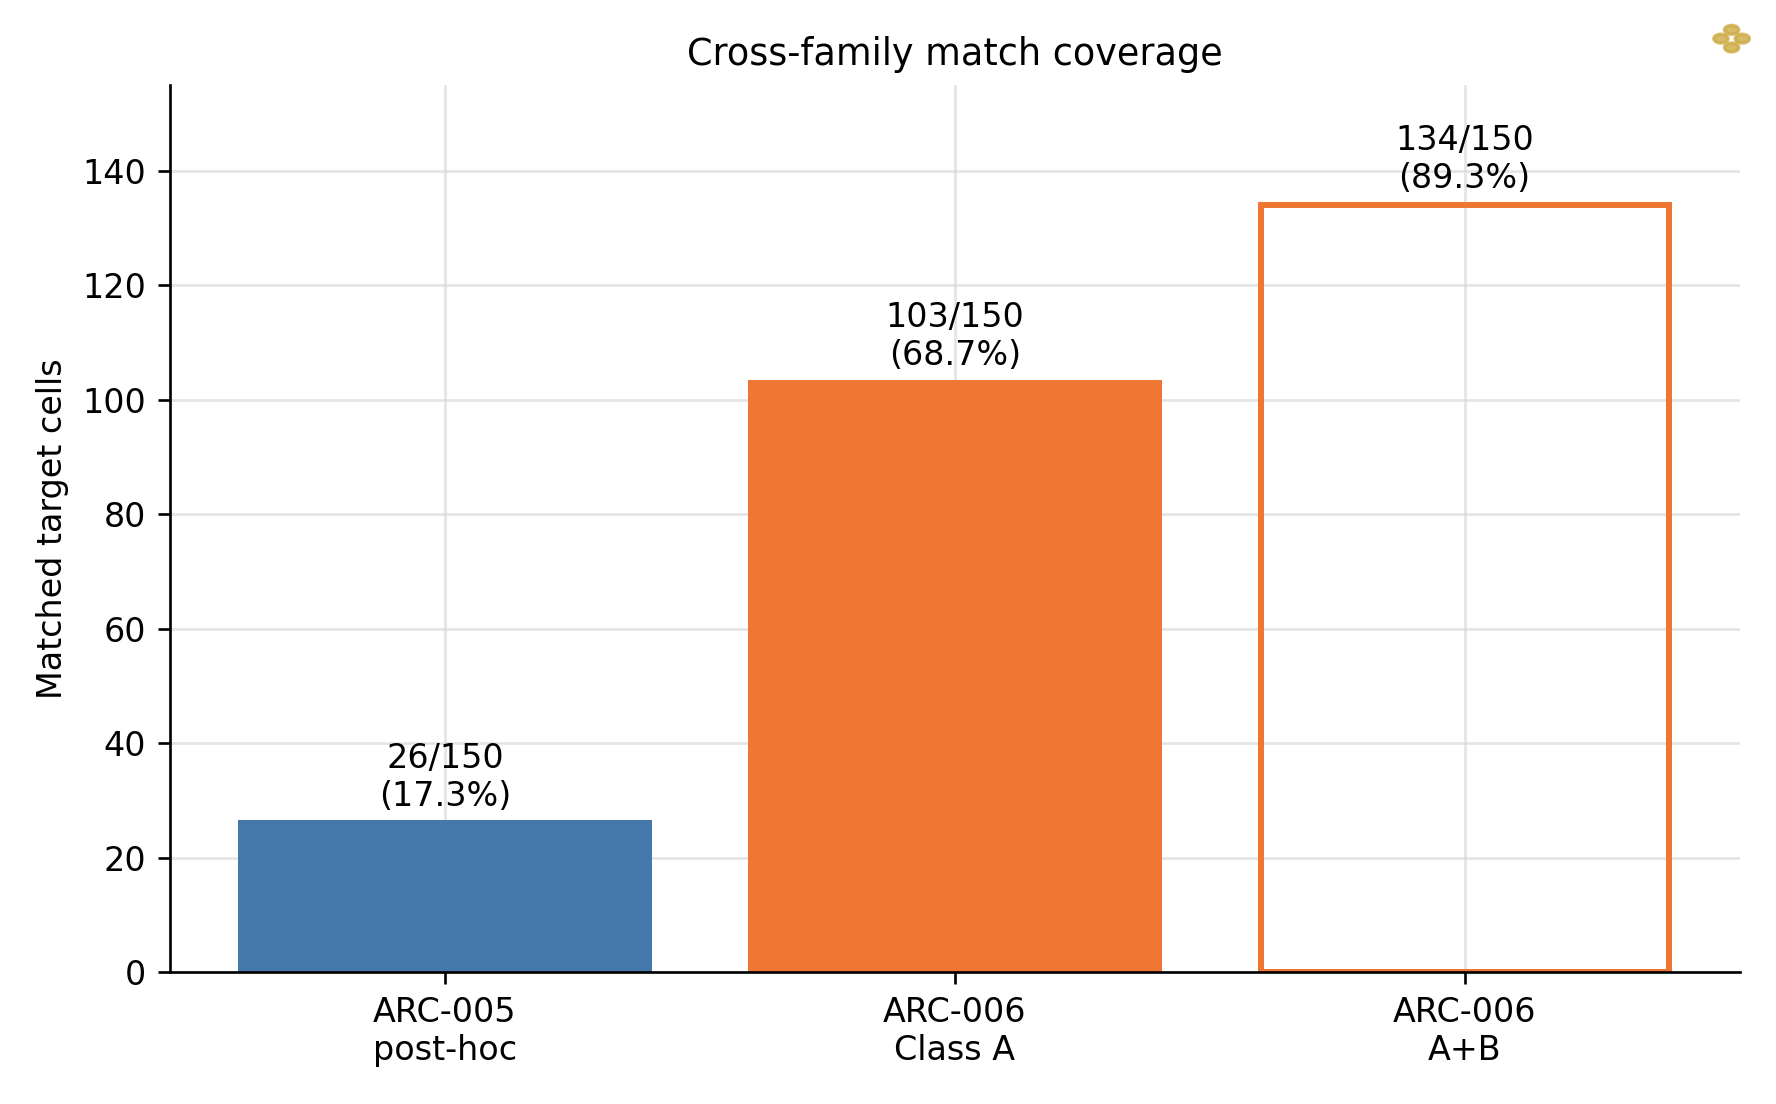
\includegraphics[width=\linewidth]{figures/draft2/fig3_match_coverage.png}
\\[-2mm]\small (a) Prospective matching support (outcome-independent)
\end{minipage}\hfill
\begin{minipage}[t]{0.50\textwidth}\centering
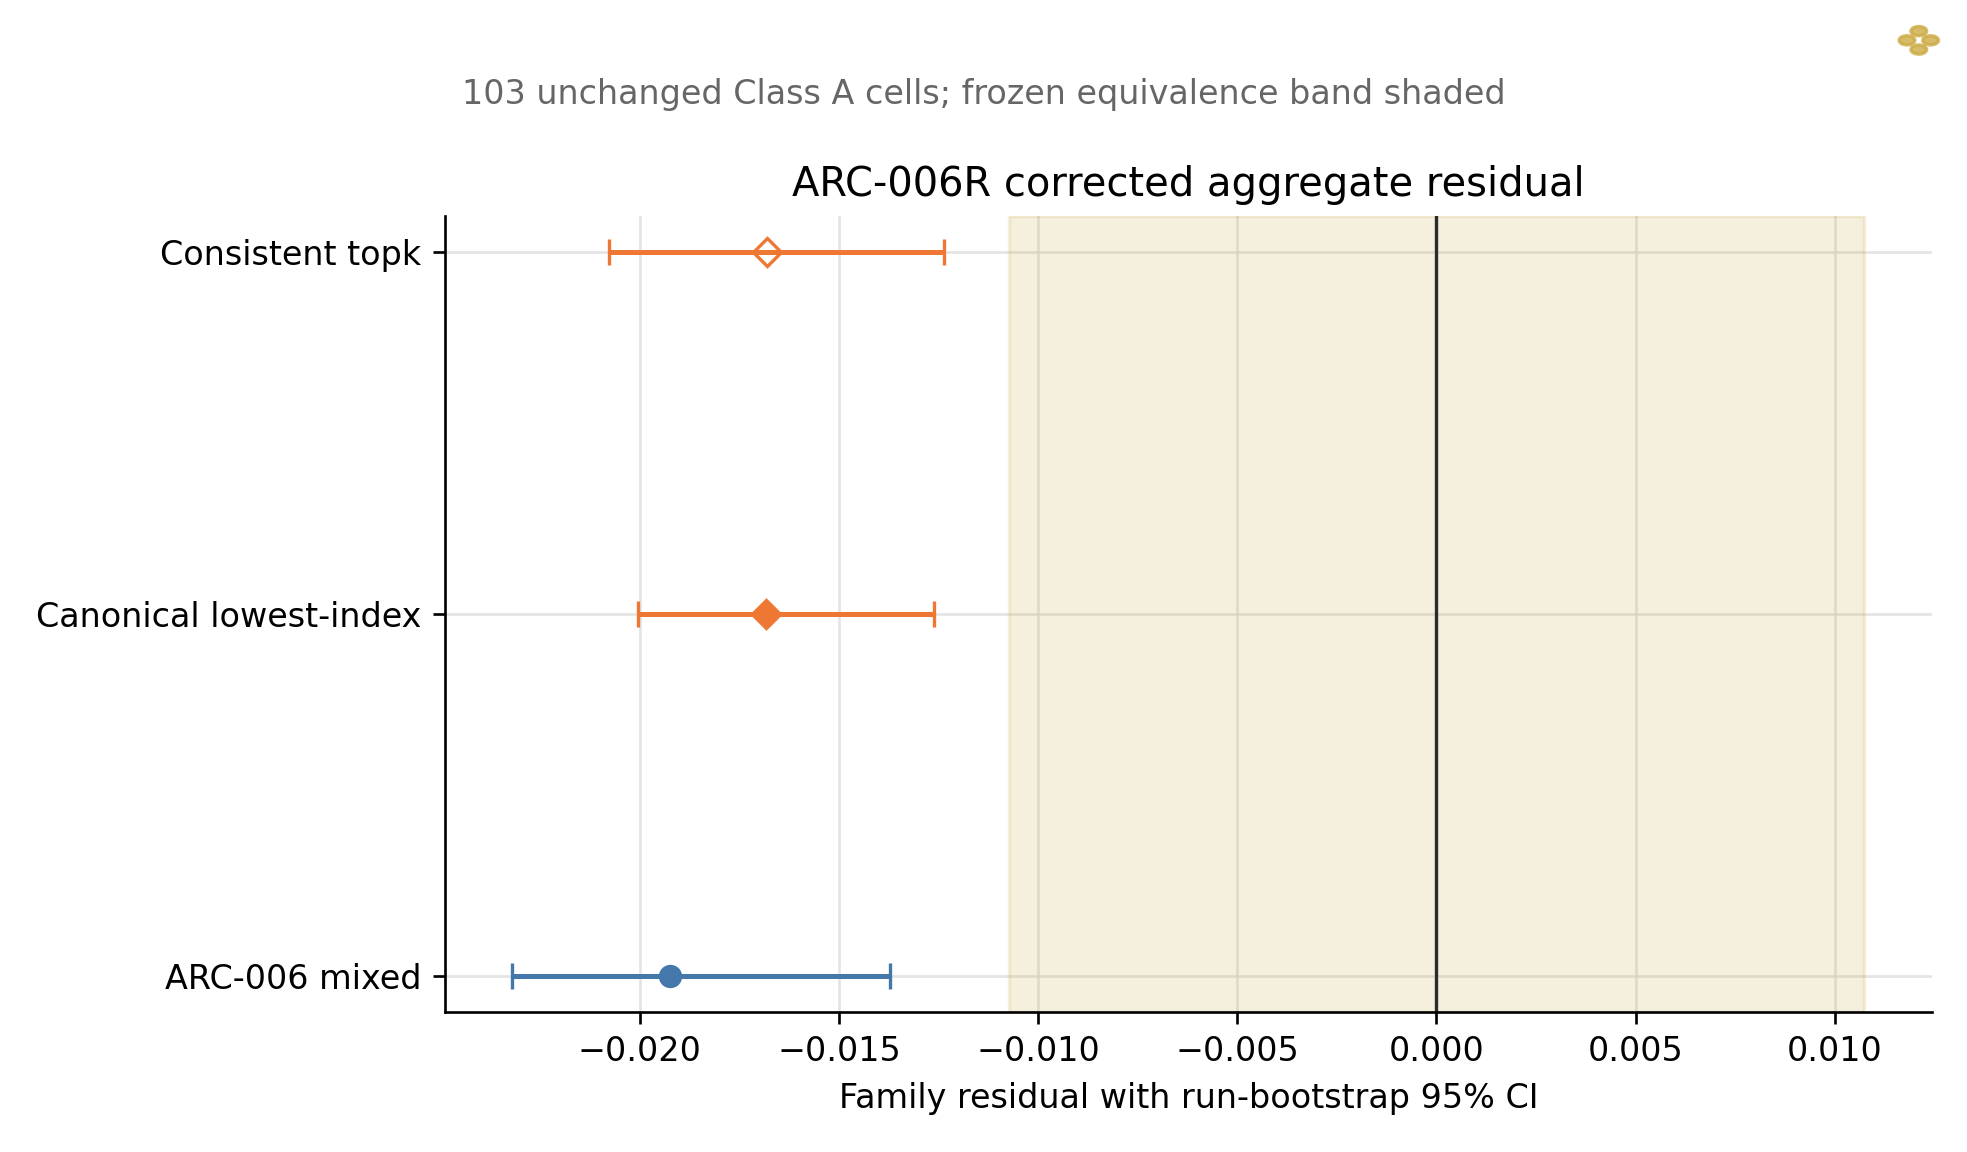
\includegraphics[width=\linewidth]{figures/draft2/fig3_corrected_residual.png}
\\[-2mm]\small (b) Corrected family residual under the canonical top-1 rule
\end{minipage}
\caption{\textbf{Predictive-damage matching does not eliminate family
dependence.} Panel (a) is a matching diagnostic and remains valid because the
assay repair did not change assignments. Panel (b) uses only corrected ARC-006R
outcomes; the withdrawn mixed-rule estimate is not shown as evidence.}
\label{fig:family}
\end{figure*}

The safe conclusion is limited but consequential: in this assay, KL and NLL
alignment is not sufficient to make the two interventions behaviorally
exchangeable. The result does not identify which unmeasured property carries
the difference.
